% Created 2017-09-29 Fri 13:32
% Intended LaTeX compiler: pdflatex
\documentclass[11pt]{article}
\usepackage[utf8]{inputenc}
\usepackage{lmodern}
\usepackage[T1]{fontenc}
\usepackage{fixltx2e}
\usepackage{graphicx}
\usepackage{longtable}
\usepackage{float}
\usepackage{wrapfig}
\usepackage{rotating}
\usepackage[normalem]{ulem}
\usepackage{amsmath}
\usepackage{textcomp}
\usepackage{marvosym}
\usepackage{wasysym}
\usepackage{amssymb}
\usepackage{amsmath}
\usepackage[version=3]{mhchem}
\usepackage[numbers,super,sort&compress]{natbib}
\usepackage{natmove}
\usepackage{url}
\usepackage{minted}
\usepackage{underscore}
\usepackage[linktocpage,pdfstartview=FitH,colorlinks,
linkcolor=blue,anchorcolor=blue,
citecolor=blue,filecolor=blue,menucolor=blue,urlcolor=blue]{hyperref}
\usepackage{attachfile}
\usepackage[left=1in, right=1in, top=1in, bottom=1in, nohead]{geometry}
\usepackage{fancyhdr}
\usepackage{hyperref}
\usepackage{setspace}
\usepackage[labelfont=bf]{caption}
\usepackage{amsmath}
\usepackage{amssymb}
\usepackage{enumerate}
\usepackage[parfill]{parskip}
\date{Due: 09-29-2017 Fri}
\title{}
\begin{document}

\title{Computational Chemistry Homework 2}
\author{Gray Laughlin, Jeonghyun Ko, Yujia Wang}
\maketitle

\section{Lectures 1-2: Review of quantum mechanics}
\label{sec:orge016894}
An electron is trapped in a \uline{one-dimensional} box described by the potential (recall 1 bohr = 0.529177 Å, is the atomic unit of length):

\begin{center}
V(x)= 
\begin{cases}
    0, & -1  < x < 1  \text{ bohr} \\
    \infty, & x \leq -1 \text{ or } x \geq 1  \text{ bohr}
\end{cases}
\end{center}

\begin{enumerate}[(a)]
\item Using the energy expression given in class, calculate the ground state (n=1) energy of the electron, in Hartree (the atomic unit of energy), in eV, and in kJ mol\(^{\text{–1}}\).
\end{enumerate}

\begin{center}

$E = \frac{n^{2}\pi^{2}\hbar^{2}}{2m_{e}L^{2}}$

For an electron in its ground state, n=1.
In atomic units \hbar = m_{e} = 1.

$E_{ground} = \frac{\pi^{2}}{(2)(2)^{2}}$
1 hartree = 27.212 eV = 2625.50 kJ mol$^{-1}$
$E_{ground} = 1.2337$ Hartree $= 33.5707$ eV $= 3239.1 $kJ mol^_{-1}

\end{center}

\begin{enumerate}[(b)]
\item We found in class that the ground-state wavefunction for this electron is \(\psi_{1}(x) = cos (\pi x/2)\). Sketch this wavefunction and show that it obeys the proper boundary conditions, has zero nodes, and is normalized.
\end{enumerate}

\begin{minted}[frame=lines,fontsize=\scriptsize,linenos]{python}
import matplotlib.pyplot as plt
import numpy as np

x = np.linspace(-1,1,30)
f = np.cos(np.pi*x/2)

plt.figure()
plt.plot(x,f)
plt.ylabel('$\psi(x)$')
plt.xlabel('X')
plt.savefig('./fig1.png')
plt.show()
\end{minted}

\begin{center}
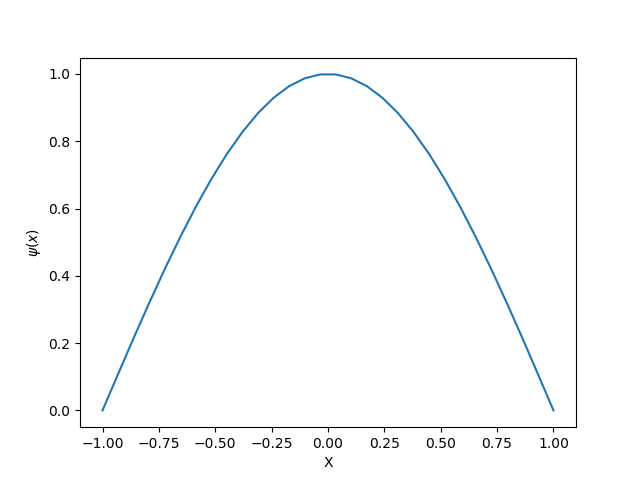
\includegraphics[width=.9\linewidth]{./fig1.png}
\end{center}

The wavefunction plot shows zero nodes because it only intersects the x-axis at the bounds. The boundary conditions were that the wavefuction must go to zero when x is greater than 1 or less than -1, because the potential energy goes to infinity in this range. The wavefunction satisfies this as shown in the plot. We can test for normalization by taking an inner product over the bounds. 

\begin{minted}[frame=lines,fontsize=\scriptsize,linenos]{python}
import numpy as np
from scipy.integrate import quad

# Normalizing
def integrand(x):
    return np.cos(np.pi * x / 2) ** 2

ans, err = quad(integrand, -1, 1)
print(ans)
\end{minted}

\begin{verbatim}
1.0
\end{verbatim}

\begin{center}

$\left \langle \psi_{1} | \psi_{1} \right \rangle = 
\int_{-\infty}^{\infty} cos^{2}(\frac{\pi x}{2}) dx = 1
$
\end{center}

\begin{enumerate}[(c)]
\item Suppose you approximate the true ground-state wavefunction by \(\phi_{1}(x) = 1 - x^{2}\). Calculate the expectation value of the energy (in Hartree) for this approximation. How does your answer compare to the energy you calculated in (a)?
\end{enumerate}

\begin{center}

The expectation value of total energy of the ground state electron is given as:
\left \langle E \right \rangle = \frac{{\left \langle \phi | \hat{H} | \phi \right \rangle}}{{\left \langle \phi | \phi \right \rangle}}

By approximating the true wavefunction as $\phi_{1}(x) = 1 - x^{2}$ and using the bounds x = [-1,1]:

${\left \langle \phi | \hat{H} | \phi \right \rangle} = \frac{8}{3}$ Hartree

Where $\hat{H}$ is the 1D kinetic energy operator, $-\frac{1}{2} \frac{\partial^_{2}}{\partial x^{2}}$.

${\left \langle \phi | \phi \right \rangle} = \frac{16}{15}$ Hartree

$\left \langle E \right \rangle = \frac{5}{4} $ Hartree

\end{center}

Or we normalize the wavefunction first \(\phi_{1}(x) = 1 - x^{2}\): \(\tilde{\phi}_{1}(x)= \left(\frac{1}{\left<\phi_1|\phi_1\right>}\right)^{1/2}\phi_1\). The expectation value of the energy can then be calculated using the Hamiltonian operator as \(\left<E\right> = \left<\tilde{\psi}|H|\tilde{\psi}\right>\).

\begin{minted}[frame=lines,fontsize=\scriptsize,linenos]{python}
import numpy as np
from scipy.integrate import quad

# Normalizing
def integrand(x):
    return (1 - x ** 2) ** 2

c, err = quad(integrand, -1, 1)

# The wavefunction can also be written as a polynomial
# (-1*x^2 + 0*x + 1) / sqrt(c)
p = 1 / np.sqrt(c) * np.array([-1, 0, 1])

def func(x):
    return -0.5 * 1 / np.sqrt(c) * (1 - x ** 2) * np.polyder(np.polyder(p)) # np.polyder(p) calculates the first derivative of p

E, err = quad(func, -1, 1)

print ('The expectation value of the energy is {0:.2f} hartree.'.format(E))
\end{minted}

\begin{verbatim}
The expectation value of the energy is 1.25 hartree.
\end{verbatim}

The energy is 1.3 \% greater than the energy in part (a).

\begin{enumerate}[(d)]
\item Can you guess an even better approximate wavefunction? Guess a candidate, evaluate the expectation value of its energy, and compare to question (c). Did you do any better than my guess?
\end{enumerate}

Linear combination of two functions helps to get better approximate wavefunction. The wavefunction has to obey the boundary conditions.

\begin{center}

The expectation value of total energy of the ground state electron is given as:
\left \langle E \right \rangle = \frac{{\left \langle \phi | \hat{H} | \phi \right \rangle}}{{\left \langle \phi | \phi \right \rangle}}

By approximating the true wavefunction with the function, $\phi_{1}(x) = (1 - x^{2}) + (1 - x^{4})$, we might be able to get a more accurate energy estimation. 

${\left \langle \phi | \hat{H} | \phi \right \rangle} = \frac{716}{105}$ Hartree

${\left \langle \phi | \phi \right \rangle} = \frac{1552}{315}$ Hartree

$\left \langle E \right \rangle =  1.384$ Hartree

The new basis function did not work as well as $1 - x^{2}$. 

\end{center}

Another try: Let \(\psi_{1}(x) = c_{1}(1-x^{2}) + c_{2}(1-x^{4})\) and set c1 = 1.2.
After normalization, we can get c2 = -0.203293.
\begin{minted}[frame=lines,fontsize=\scriptsize,linenos]{python}
import numpy as np
from scipy.integrate import quad
from sympy import Symbol, Derivative
x= Symbol('x')
hbar = 1
m = 1

def integrand(x):
    return (1.2 * (1 - x**2) - 0.203293 * (1 - x**4)) * (-hbar ** 2)/(2 * m) * (-2.4 + 2.43952 * x**2) 

soln = quad(integrand, -1, 1)

print ('The expectation value of the energy = {0:1.4f} Hartree.'.format(soln[0]))
\end{minted}

The expectation value of the energy = 1.2338 Hartree.

The energy is very close to the energy in part (a) (1.2337 Hartree).


\section{Lectures 3: Many-electron atoms}
\label{sec:org6482b9f}

Hartree’s father performed the first calculations on multi-electron atoms by hand. Today those same calculations (much better ones, in fact) can be done in the blink of an eye on a computer. In this problem you will use a code first developed by Herman and Skillman in the 1960’s to calculate the wavefunctions and energy of an atom using the Hartree-Fock-Slater (HFS) model, an early predecessor to DFT. The necessary software, rewritten in \texttt{C++}, is available at \texttt{/afs/crc.nd.edu/users/w/wschnei1/CBE547/fda.tar.gz}.

Copy the software to your home directory, unpack (\texttt{tar –xzf fda.tar.gz}), change into the directory (\texttt{cd fda}) and compile the code(\texttt{make fda}) to create the fda executable. Look at the \texttt{00README} file for information about the computer program and the format of the input. If you are brave, glance through the various source files (\texttt{*.cxx}) to get a sense of what the code is doing. Note that the code uses atomic units, Hartree for energy and bohr for distance.

\begin{enumerate}[(a)]
\item Run the \texttt{Ar.inp} example included in the directory (\texttt{fda Ar}). If all goes well, you should get an output file (\texttt{Ar.out}) and a dump file (\texttt{Ar.dmp}). Look at the \texttt{Ar.out} file to answer these questions:

\begin{itemize}
\item How many self-consistent field (SCF) iterations does the calculation take to converge?

\item What is the final calculated HFS energy of the atom?

\item What are the identities (1s, 2p, etc.) and energies of the occupied atomic orbitals?
\end{itemize}
\end{enumerate}

output
\begin{minted}[frame=lines,fontsize=\scriptsize,linenos]{python}
itr = 29
  l = 0
    n = 1, e =    -116.93655734 (   -233.87311468)
    n = 2, e =     -11.60370286 (    -23.20740572)
    n = 3, e =      -1.10223823 (     -2.20447646)
  l = 1
    n = 2, e =      -9.27212718 (    -18.54425437)
    n = 3, e =      -0.57350833 (     -1.14701666)
  cnv =   0.000009, mix =   0.499982
  integrated charge =  17.999977 out of  18.000000

                   Orbital Summary
 nl    occ        E           KE       <1/r>     <r>
 1s   2.00    -116.9366    155.6552   17.6458   0.0856
 2s   2.00     -11.6037     25.6407    3.5930   0.4087
 2p   6.00      -9.2721     25.0012    3.5259   0.3675
 3s   2.00      -1.1022      4.4193    1.0227   1.3584
 3p   6.00      -0.5735      3.4406    0.8812   1.5596

     Energy Summary
 kinetic energy      =   542.0811
 potential energy    = -1068.9087
 one-electron energy =  -735.2963
 two-electron energy =   208.4688

 total energy =  -526.8275
 virial ratio =    -1.9719
\end{minted}

It takes 29 iteration steps to converge.

The final calculated HFS energy of the atom is -526.8275 Hartree.

The identities and the energies of the occupied atomic orbitals orbital energies are here below.

\begin{center}
\begin{tabular}{lrrrrr}
nl & occ & E & KE & <1/r> & <r>\\
\hline
1s & 2 & -116.9366 & 155.6552 & 17.6458 & 0.0856\\
2s & 2 & -11.6037 & 25.6407 & 3.593 & 0.4087\\
2p & 6 & -9.2721 & 25.0012 & 3.5259 & 0.3675\\
3s & 2 & -1.1022 & 4.4193 & 1.0227 & 1.3584\\
3p & 6 & -0.5735 & 3.4406 & 0.8812 & 1.5596\\
\end{tabular}
\end{center}

\begin{enumerate}[(b)]
\item The fda code solves the HFS equations on a radial grid. The \texttt{Ar.dmp} file contains the radial grid values and the total charge density in two columns of length 300, followed by an output of each orbital on the same grid. Plot out the charge density and each of the orbitals.
\end{enumerate}

See plots
\begin{minted}[frame=lines,fontsize=\scriptsize,linenos]{python}
import matplotlib.pyplot as plt
import numpy as np

# Lets open the file in read mode
with open('FDA/Ar/Ar.dmp', 'r') as f:

    # Read all the lines
    lines = f.readlines()

    # made list of grid points and total charge densities
    grid_points = []
    total_charge_densities = []

    for line in lines[3:303]:

        # split the lines into two columns
        grid_point, tot_charge_density = line.split()

        # We need to convert each line to a float add it to our lists
        # store the each data in the lists
        grid_points.append(float(grid_point))
        total_charge_densities.append(float(tot_charge_density))

    # Now the individual orbitals
    one_s_charge_density = [float(x) for x in lines[304:604]]
    two_s_charge_density = [float(x) for x in lines[605:905]]  
    two_p_charge_density = [float(x) for x in lines[906:1206]]
    three_s_charge_density = [float(x) for x in lines[1207:1507]]
    three_p_charge_density = [float(x) for x in lines[1508:1808]]
  
# plot the total charge densities
plt.figure()
plt.semilogx(grid_points, total_charge_densities)
plt.xlabel('Grid Points')
plt.ylabel('Charge Density')
plt.title('Overall')
plt.savefig('Ar-overall-charge-density.png')

# plot the individual orbitals
plt.figure()
plt.semilogx(grid_points, one_s_charge_density, label='1s')
plt.semilogx(grid_points, two_s_charge_density, label='2s')
plt.semilogx(grid_points, two_p_charge_density, label='2p')
plt.semilogx(grid_points, three_s_charge_density, label='3s')
plt.semilogx(grid_points, three_p_charge_density, label='3p')
plt.xlabel('Grid Points')
plt.ylabel('Charge Density')
plt.title('Individual')
plt.xlim(min(grid_points), max(grid_points))
plt.legend()
plt.savefig('Ar-orbital-charge-density.png')
plt.show()
\end{minted}

\begin{center}
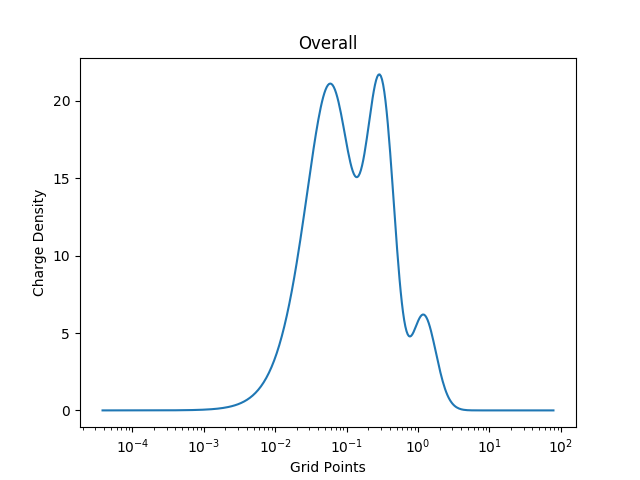
\includegraphics[width=.9\linewidth]{./Ar-overall-charge-density.png}
\end{center}
\begin{center}
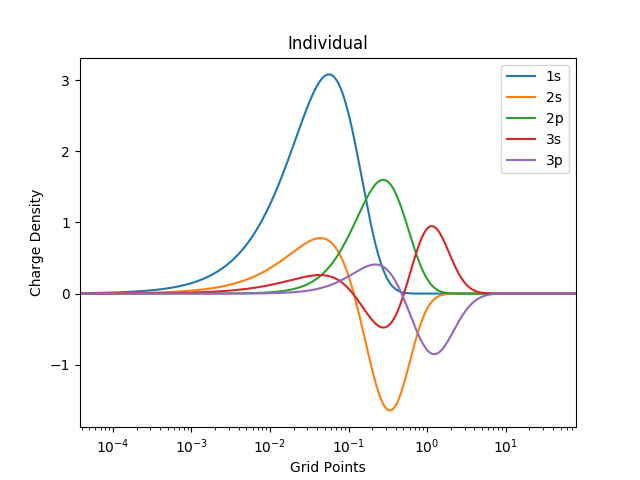
\includegraphics[width=.9\linewidth]{./Ar-orbital-charge-density.png}
\end{center}

\begin{enumerate}[(c)]
\item Choose one of the d block atoms. From the periodic table, figure out its electronic configuration and create an fda input file for it (follow the instructions in \texttt{00README} for how to specify the atomic number and the orbital occupancies of your atom). Run the fda calculation on your atom.

\begin{itemize}
\item What is the final calculated HFS energy of the atom? How does it compare to Ar?

\item What are the identities (1s, 2p, etc.) and energies of the occupied atomic orbitals?
\end{itemize}
\end{enumerate}


\begin{itemize}
\item We chose Cu as an example. The electron configuration of Cu is \(1s^{2} 2s^{2} 2p^{6} 3s^{2} 3p^{6} 3d^{10} 4s^{1}\). After 30 iteration steps, the calculation was converged.
\end{itemize}

input
\begin{minted}[frame=lines,fontsize=\scriptsize,linenos]{python}
300 0.0001 30.0
50 0.00001 0.10 0.50  0.682 0.0042
29.0 7
1 0 1.0 1.0
2 0 1.0 1.0
2 1 3.0 3.0
3 0 1.0 1.0
3 1 3.0 3.0
3 2 5.0 5.0
4 0 1.0 0.0
\end{minted}


output
\begin{minted}[frame=lines,fontsize=\scriptsize,linenos]{python}
                   Orbital Summary
 nl    occ        E           KE       <1/r>     <r>
 1s   2.00    -325.9926    409.2882   28.6152   0.0527
 2s   2.00     -39.3532     78.0568    6.2572   0.2363
 2p   6.00     -34.7802     77.8063    6.2308   0.2051
 3s   2.00      -4.4010     17.1817    1.9870   0.7120
 3p   6.00      -2.9273     15.4940    1.8626   0.7384
 3d  10.00      -0.4205     10.4720    1.4713   0.9331
 4s   1.00      -0.2645      1.1132    0.4398   2.9912

     Energy Summary
 kinetic energy      =  1674.6889
 potential energy    = -3315.2096
 one-electron energy = -2310.8336
 two-electron energy =   670.3128

 total energy = -1640.5208
 virial ratio =    -1.9796
\end{minted}


The final calculated HFS energy of the Cu atom is -1640.5208 Hartree.

It is about 3.11 times the total energy of Ar atom.

The identities and the energies of the occupied atomic orbitals orbital energies are here below.

\begin{center}
\begin{tabular}{lrrrrr}
nl & occ & E & KE & <1/r> & <r>\\
\hline
1s & 2 & -325.9926 & 409.2882 & 28.6152 & 0.0527\\
2s & 2 & -39.3532 & 78.0568 & 6.2572 & 0.2363\\
2p & 6 & -34.7802 & 77.8063 & 6.2308 & 0.2051\\
3s & 2 & -4.401 & 17.1817 & 1.987 & 0.712\\
3p & 6 & -2.9273 & 15.494 & 1.8626 & 0.7384\\
3d & 10 & -0.4205 & 10.472 & 1.4713 & 0.9331\\
4s & 1 & -0.2645 & 1.1132 & 0.4398 & 2.9912\\
\end{tabular}
\end{center}


\begin{enumerate}[(d)]
\item The orbital energies are a rough approximation of the energy to remove an electron from that orbital. Use your result to estimate the first ionization energy of your atom. How does it compare with the experimental first ionization energy?
\end{enumerate}

The experimental first ionization energy of Cu is 745.5 kJ/mol (ref. \url{https://www.webelements.com/copper/atoms.html})

From our HFS result, the estimated first ionization energy of Cu is 0.2645 Hartree (= 694.4 kJ/mol). 

There is a 6.85 \% difference from the experimental result.

\begin{enumerate}[(e)]
\item You can also do calculations on anions or cations. Modify the input file for your atom by removing one of the valence electrons, to make it a cation. Rerun fda on the cation. 

\begin{itemize}
\item How does the HFS energy of the cation compare to the neutral metal atom?
\item Do the energies of the orbitals go up or down from the neutral to the cation?
\item Do the electrons get closer to or further from the nucleus in the cation compared to the neutral? Use the expectation values of the distances from the nucleus (<r>) to answer the question.
\end{itemize}
\end{enumerate}

input
\begin{minted}[frame=lines,fontsize=\scriptsize,linenos]{python}
300 0.0001 30.0
50 0.00001 0.10 0.50  0.682 0.0042
29.0 6
1 0 1.0 1.0
2 0 1.0 1.0
2 1 3.0 3.0
3 0 1.0 1.0
3 1 3.0 3.0
3 2 5.0 5.0
\end{minted}

output
\begin{minted}[frame=lines,fontsize=\scriptsize,linenos]{python}
                   Orbital Summary
 nl    occ        E           KE       <1/r>     <r>
 1s   2.00    -326.3601    409.2915   28.6154   0.0527
 2s   2.00     -39.7146     78.0586    6.2573   0.2363
 2p   6.00     -35.1421     77.8096    6.2309   0.2051
 3s   2.00      -4.7657     17.1741    1.9866   0.7121
 3p   6.00      -3.2918     15.4907    1.8625   0.7383
 3d  10.00      -0.7824     10.5383    1.4778   0.9229

     Energy Summary
 kinetic energy      =  1674.2338
 potential energy    = -3314.5026
 one-electron energy = -2300.4296
 two-electron energy =   660.1608

 total energy = -1640.2688
 virial ratio =    -1.9797
\end{minted}

\begin{itemize}
\item The total energy of Cu cation is -1640.2688  Hartree which is 0.252 Hartree higher than that of neutral Cu (-1640.5208 Hartree).
\item All orbital energies of Cu cation decrease
\item The average distances of 3d orbitals from the nucleus is decreased. The change of the average distance of the others are marginal.
\end{itemize}

\begin{enumerate}[(f)]
\item The difference in total energy between your neutral and cation calculations is another estimate of the first ionization energy of your atom. How does this estimate compare with experiment?
\end{enumerate}
The estimated first ionization energy of Cu is 0.2645 Hartree.

But the the energy difference between Cu and Cu+ is 0.252 Hartree.

very close!
\end{document}